% ============================================================================
%  Phase I Report -- Write-Back Cache Controller (IEEE conference format)
%  Compile on Overleaf (pdfLaTeX) or locally:  pdflatex report && pdflatex report
%  Figures are read from ../docs/figures/ (copy that folder next to this file
%  on Overleaf and change \graphicspath if needed).
% ============================================================================
\documentclass[conference]{IEEEtran}
\IEEEoverridecommandlockouts
\usepackage{cite}
\usepackage{amsmath,amssymb}
\usepackage{graphicx}
\usepackage{booktabs}
\usepackage{array}
\usepackage{xcolor}
\usepackage[hidelinks]{hyperref}
\graphicspath{{../docs/figures/}{figures/}}

\begin{document}

\title{Design and Verification of a Direct-Mapped\\Write-Back Cache Controller in Verilog HDL\\
{\large Phase I Report -- Modern Computer Architecture, Project 8}\\ {\large\itshape Group: Khel Khatam}}

\author{
\IEEEauthorblockN{Pankaj Upadhyay}
\IEEEauthorblockA{Roll No. 2401010317\\ MCA}
\and
\IEEEauthorblockN{Prakhar Rawat}
\IEEEauthorblockA{Roll No. 2401020045\\ MCA}
\and
\IEEEauthorblockN{Harshit Kudhial}
\IEEEauthorblockA{Roll No. 2401010182\\ MCA}
\and
\IEEEauthorblockN{Om Chimurkar}
\IEEEauthorblockA{Roll No. 2401010306\\ MCA}
\and
\IEEEauthorblockN{Vishuti Jamwal}
\IEEEauthorblockA{Roll No. 2401010506\\ MCA}
}

\maketitle

\begin{abstract}
Main-memory bandwidth is a scarce resource, and every store that a cache forwards
to memory consumes it. This project designs, implements and verifies a
direct-mapped \emph{write-back, write-allocate} cache controller in synthesizable
Verilog HDL. The design is partitioned into a Cache Data RAM, Tag RAM, Valid RAM,
Dirty-Bit RAM, Tag Comparator, a four-state controller FSM (\textsc{Idle},
\textsc{Compare}, \textsc{Write-Back}, \textsc{Allocate}) and a block-transfer
Memory Interface. A dirty bit per line records whether the cached block differs
from memory, so write hits are absorbed by the cache and a block is written to
memory only when a dirty line is evicted---strictly \emph{before} the new block is
refilled. A write-through, no-write-allocate cache with identical geometry is
built as a reference. A self-checking directed testbench with a golden memory
model executes 6\,494 checks with zero failures and covers all four controller
states and all six legal transitions. On workloads with temporal write locality
the write-back cache moves 78--88\% fewer words to and from memory and finishes
3.7--3.8$\times$ faster than the write-through cache, while streaming and
conflict-heavy store patterns expose the cost of write-allocation, which motivates
the Phase II improvements.
\end{abstract}

\begin{IEEEkeywords}
cache memory, write-back, write-through, dirty bit, cache controller, finite state
machine, Verilog HDL, memory traffic
\end{IEEEkeywords}

% ----------------------------------------------------------------------------
\section{Introduction}
The gap between processor and DRAM speed makes the cache hierarchy the main lever
for performance and for memory-bandwidth consumption~\cite{hp_quant,jacob}.
Besides deciding \emph{what} to keep, a cache must decide \emph{when} a store
reaches main memory. A \emph{write-through} cache forwards every store,
which keeps memory always up to date but generates one bus transaction per store.
A \emph{write-back} cache updates only its own copy and marks the line
\emph{dirty}; memory is updated once, when the dirty line is replaced. Repeated
stores to the same block therefore cost a single block write~\cite{smith82,goodman83}.

The price of write-back is controller complexity: a miss that selects a dirty
victim must first transfer the old block to memory and only then refill the line,
and the dirty bit must be set, cleared and tested at exactly the right moments.
This project implements that controller in RTL and checks it against a
write-through baseline.

\textbf{Objectives.} (i)~Implement read hits and misses; (ii)~implement write hits
using dirty bits; (iii)~handle dirty-block eviction, writing the old block to memory
before refill; (iv)~verify every controller state and transition; and (v)~compare
memory traffic against write-through behaviour.

% ----------------------------------------------------------------------------
\section{Literature Review}
\textbf{Cache fundamentals and write policies.} Smith's survey~\cite{smith82}
established the vocabulary used today: placement, replacement, line size, and
the write-through versus copy-back (write-back) choice. It observed that
write-back reduces memory traffic but complicates consistency, because memory may
hold stale data. Goodman~\cite{goodman83} studied caches specifically as a means
of reducing processor--memory traffic in shared-bus systems and showed that
copy-back caches cut bus traffic far more than write-through ones, the starting
point of later snooping-coherence protocols.

\textbf{Write-miss policies.} Jouppi~\cite{jouppi93} separated the write-hit
policy (write-through or write-back) from the write-miss policy (fetch-on-write,
write-allocate, write-validate, write-around, write-invalidate). He showed that
write-back with fetch-on-write reads blocks that are about to be overwritten
entirely, and that no-fetch-on-write variants with per-word valid bits remove
much of that traffic. This is exactly the effect our streaming-store experiment
reproduces (Section~\ref{sec:prelim}).

\textbf{Direct-mapped organisation.} Hill~\cite{hill88} argued that direct-mapped
caches, despite higher miss ratios, can win on access time and simplicity because
the tag check and data read happen in parallel with no way-selection multiplexer.
Jouppi~\cite{jouppi90} showed that their main weakness, conflict misses, can be
reduced with small victim caches. We use direct mapping for the Phase I prototype
and use a conflict-thrash workload to measure that weakness.

\textbf{Controller design.} Patterson and Hennessy~\cite{ph_cod} give the classic
four-state FSM for a simple write-back cache (Idle, Compare Tag, Write-Back,
Allocate) with a blocking CPU interface and a multi-cycle memory. Our controller
follows that structure. Hennessy and Patterson~\cite{hp_quant} and Jacob
\emph{et~al.}~\cite{jacob} quantify the benefits of write buffers, dirty bits and
write-back in modern memory hierarchies.

\textbf{Write-back scheduling in modern systems.} In current last-level caches the
question is \emph{when} dirty data is written back. Eager write-back~\cite{lee00}
writes dirty lines that are likely to be evicted early, while the bus is idle,
to smooth bursts. The virtual write queue~\cite{stuecheli10} coordinates
last-level-cache write-backs with DRAM scheduling to reduce read--write turnaround
penalties. These techniques still rely on the basic dirty-bit mechanism
implemented here.

\textbf{Gap addressed.} Textbooks describe the write-back FSM at the
behavioural level. This project provides a complete, modular, synthesizable RTL
implementation with a self-checking verification environment and a
cycle-accurate, word-level traffic comparison against write-through using the same
datapath blocks.

% ----------------------------------------------------------------------------
\section{Proposed Solution}

\subsection{Cache Organisation}
The cache is direct-mapped with 16 lines of 16~bytes (four 32-bit words), giving
256~bytes of data. A 32-bit byte address is split as
\begin{equation}
\underbrace{A[31{:}8]}_{\text{tag (24)}}\;|\;
\underbrace{A[7{:}4]}_{\text{index (4)}}\;|\;
\underbrace{A[3{:}2]}_{\text{word}}\;|\;
\underbrace{A[1{:}0]}_{\text{byte}}.
\end{equation}
The policy is \emph{write-back} on write hits and \emph{write-allocate}
(fetch-on-write) on write misses. Main memory is a block-transfer model with a
fixed latency of 10 cycles per transaction. All sizes are \texttt{`define}
parameters in \texttt{cache\_params.vh}.

\begin{figure*}[t]
\centering
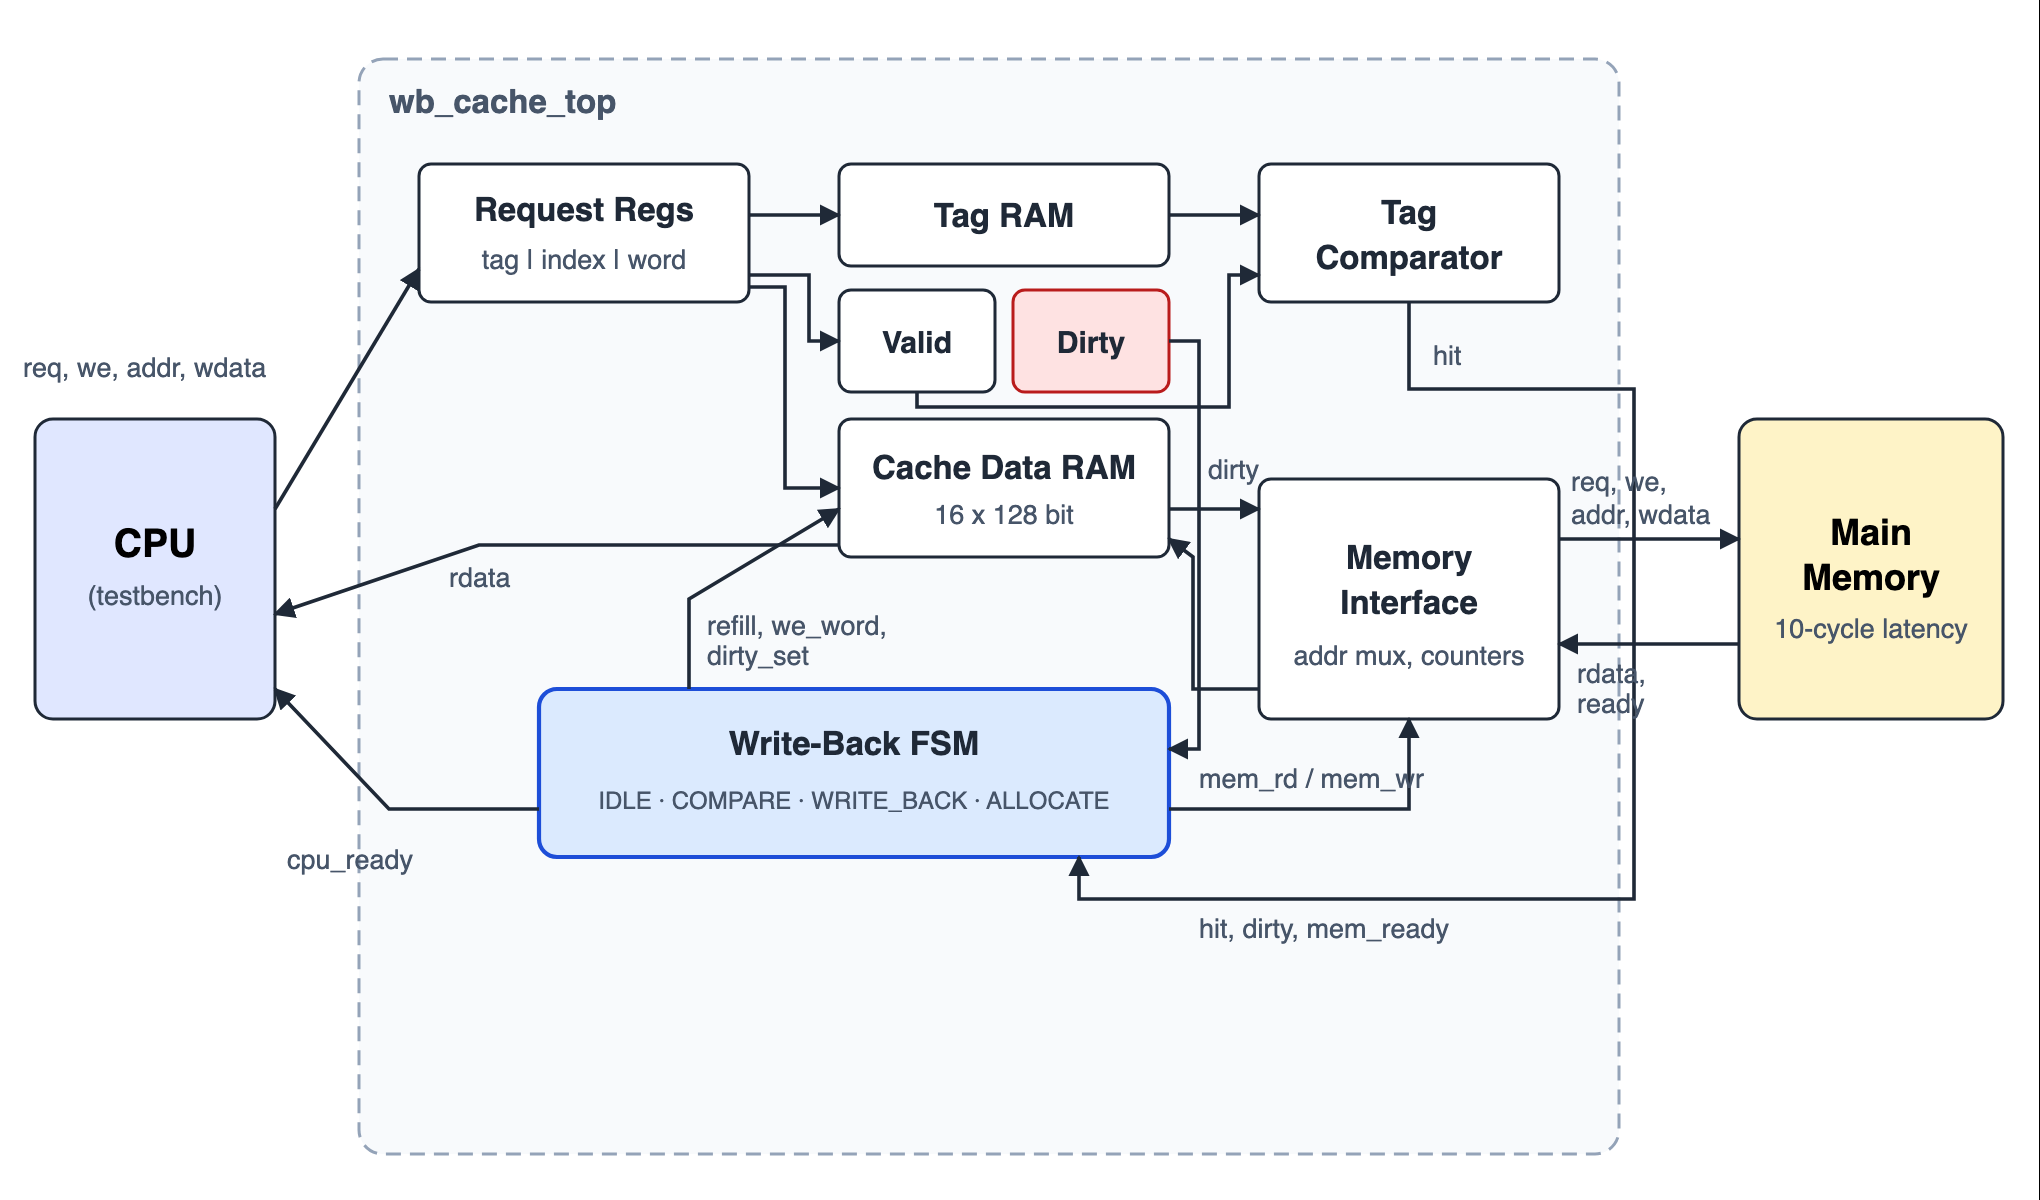
\includegraphics[width=0.72\textwidth]{fig_block.png}
\caption{Block diagram of the write-back cache (\texttt{wb\_cache\_top}).}
\label{fig:block}
\end{figure*}

\subsection{RTL Modules}
Fig.~\ref{fig:block} shows the datapath. Each suggested module is a separate
Verilog file:
\begin{itemize}
\item \textbf{Cache Data RAM} -- $16\times128$-bit array with combinational read
and synchronous write of a full line (refill) or a single word (store hit).
\item \textbf{Tag RAM} -- $16\times24$-bit array, written on refill.
\item \textbf{Valid RAM} -- 16 bits, cleared by reset, set on refill.
\item \textbf{Dirty-Bit RAM} -- 16 bits. \emph{Set} on a write hit,
\emph{cleared} on refill and on reset; clear has priority.
\item \textbf{Tag Comparator} -- $\textit{hit}=\textit{valid}\wedge
(\textit{tag}_{\text{stored}}=\textit{tag}_{\text{req}})$.
\item \textbf{Write-Back FSM} -- the controller (Section~\ref{sec:fsm}).
\item \textbf{Memory Interface} -- builds the bus request. On a write-back the
address is reconstructed from the \emph{victim} tag stored in the Tag RAM and
the current index, $\{\textit{tag}_{\text{victim}},\textit{index}\}$. On a
refill it is the requested block address. It also counts read and write
bursts.
\end{itemize}
Request registers capture address, data and R/W when a request is accepted, so
the CPU-side signals may change while the miss is serviced.

\subsection{Controller FSM}\label{sec:fsm}
\begin{figure}[t]
\centering
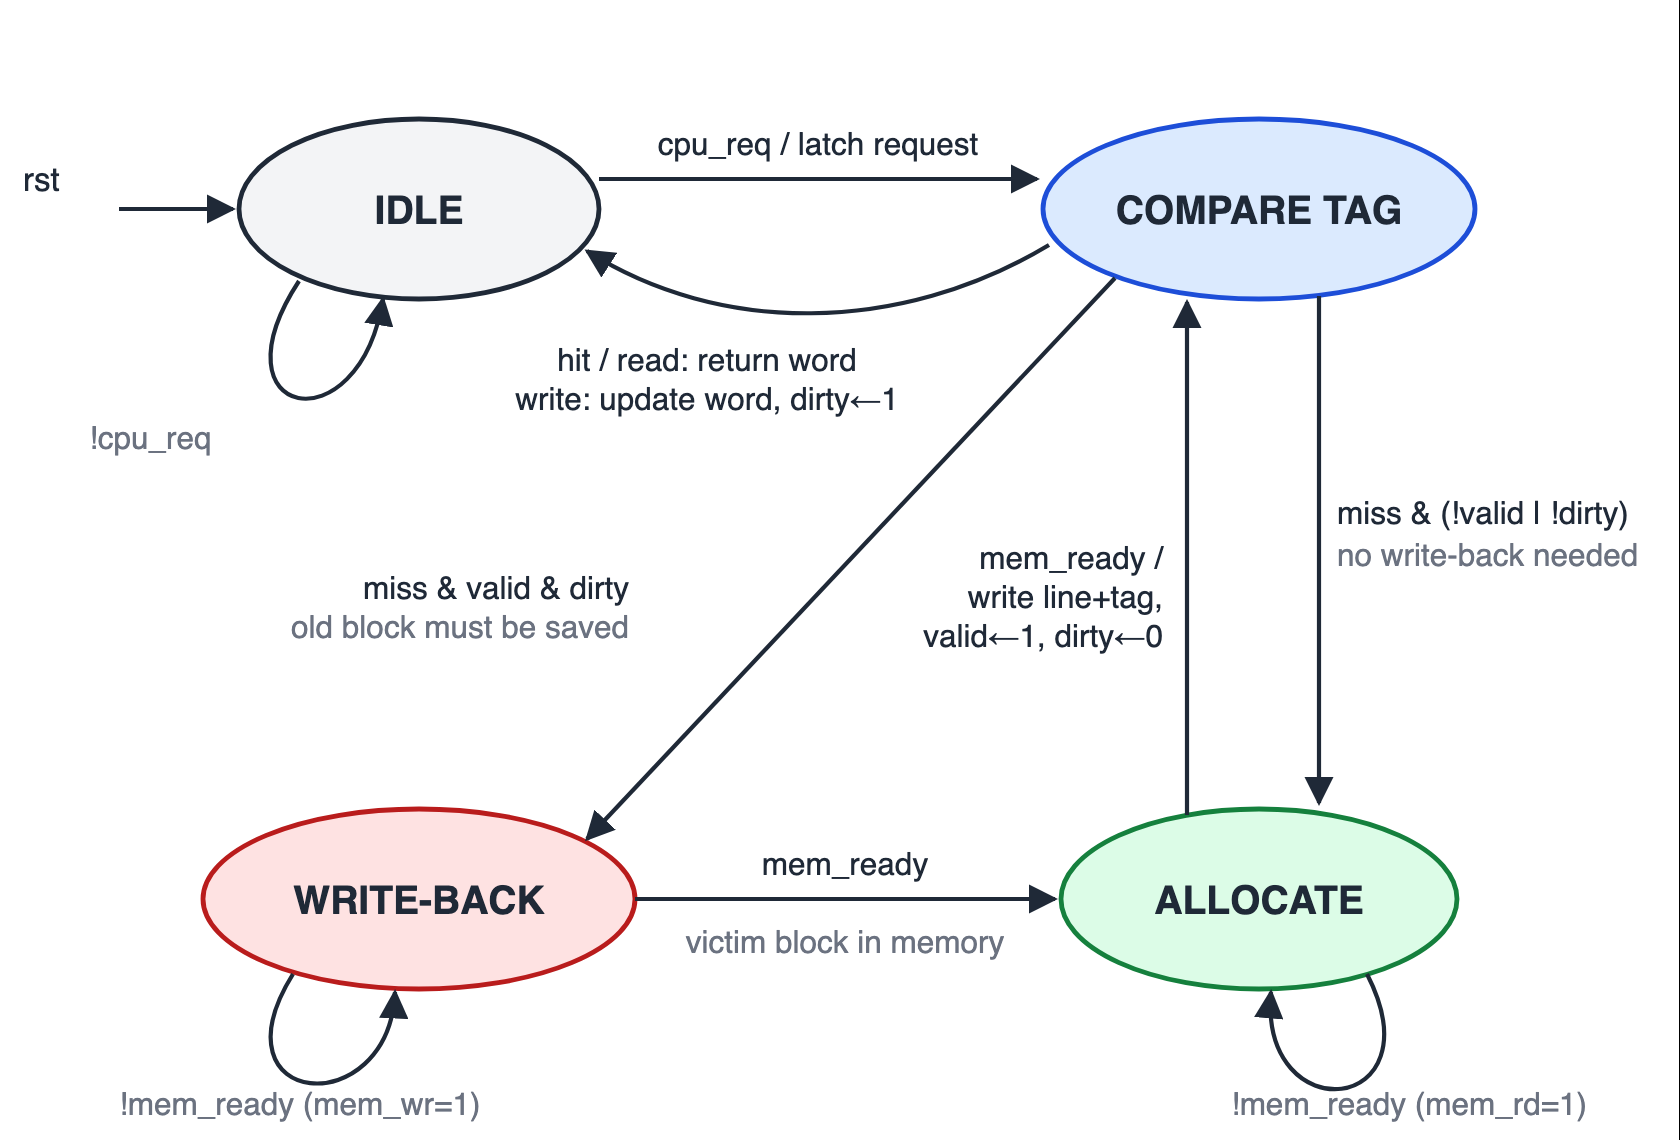
\includegraphics[width=0.92\columnwidth]{fig_fsm.png}
\caption{Write-back cache controller state diagram.}
\label{fig:fsm}
\end{figure}

Fig.~\ref{fig:fsm} gives the state diagram:
\begin{itemize}
\item \textsc{Idle}: wait for \texttt{cpu\_req}; latch the request.
\item \textsc{Compare}: on a hit, a read returns the word and a write updates
it and sets the dirty bit; both return to \textsc{Idle} (2-cycle hit latency).
On a miss, if the victim line is valid \emph{and} dirty go to
\textsc{Write-Back}, otherwise go directly to \textsc{Allocate}.
\item \textsc{Write-Back}: drive the victim block to memory and wait for
\texttt{mem\_ready}. The old data is therefore saved before it can be overwritten.
\item \textsc{Allocate}: read the requested block. On \texttt{mem\_ready} write
line and tag, set valid, clear dirty, and return to \textsc{Compare}. The
re-compare now hits and completes the original read or write, so a store miss
leaves the new line dirty.
\end{itemize}
A \texttt{first\_cmp} flag ensures that each request is counted as exactly one hit
or one miss, even though a miss passes through \textsc{Compare} twice.

\subsection{Write-Through Reference Design}
For the comparison, \texttt{wt\_cache\_top} reuses the same Data, Tag and Valid
RAMs and the Tag Comparator, without dirty bits. It is
\emph{write-through, no-write-allocate}: every store sends one word to memory
(word-masked write) and also updates the cache on a hit, while a store miss does
not allocate. It has no write buffer, so the CPU stalls on every store, the
textbook baseline~\cite{ph_cod}.

\subsection{Verification Strategy}
The testbench (\texttt{tb\_cache.v}) drives the \emph{same} request stream into
both caches, each attached to its own memory model:
\begin{itemize}
\item a \textbf{golden model} (a flat array) checks every read returned by
both caches;
\item \textbf{white-box checks} inspect the valid, dirty and tag arrays and the
memory contents after each directed test;
\item a \textbf{coherence check} after each test verifies that, for
write-back, \{cache if valid and tag-matched, otherwise memory\} equals the
golden model, and that for write-through main memory alone always equals the
golden model;
\item \textbf{FSM coverage} monitors record cycles per state, all six legal
transitions, and flag any illegal transition.
\end{itemize}

\subsection{Prototype Status and Preliminary Verification}\label{sec:prelim}
The complete RTL, reference cache, testbench and scripts are implemented and
simulate under Icarus Verilog~13~\cite{icarus} (IEEE~1364-2005
semantics~\cite{ieee1364}) with zero compile warnings.

\begin{table}[t]
\caption{Directed Tests (all pass)}
\label{tab:directed}
\centering
\footnotesize
\begin{tabular}{@{}l p{6.6cm}@{}}
\toprule
\textbf{ID} & \textbf{Scenario and checked behaviour} \\
\midrule
T0 & Reset: all lines invalid and clean, FSM in \textsc{Idle} \\
T1 & Read miss, invalid line $\rightarrow$ \textsc{Allocate} only, no write-back \\
T2 & Read hit: no memory traffic \\
T3 & Write hit: dirty set; WB memory unchanged, WT memory updated \\
T4 & 3 more writes to dirty line: 0 WB transactions vs.\ 4 WT writes \\
T5 & Read miss on dirty line: \textsc{Write-Back} \emph{then}
      \textsc{Allocate}; old data found in memory \\
T6 & Clean victim: no write-back \\
T7 & Write miss, invalid line: allocate, write, line dirty (WT: no allocate) \\
T8 & Write miss on dirty line: write-back, allocate, write \\
T9 & Read-back of written and evicted data \\
T10 & Dirty all 16 lines, sweep: exactly 16 write-backs, all clean \\
T11 & Synchronous reset clears valid, dirty and counters \\
\bottomrule
\end{tabular}
\end{table}

Table~\ref{tab:directed} lists the directed tests. The full run (directed tests
plus seven workloads) executes \textbf{6\,494 checks with 0 errors}. The FSM
visits all four states and all six legal transitions with no illegal ones.

\begin{figure*}[t]
\centering
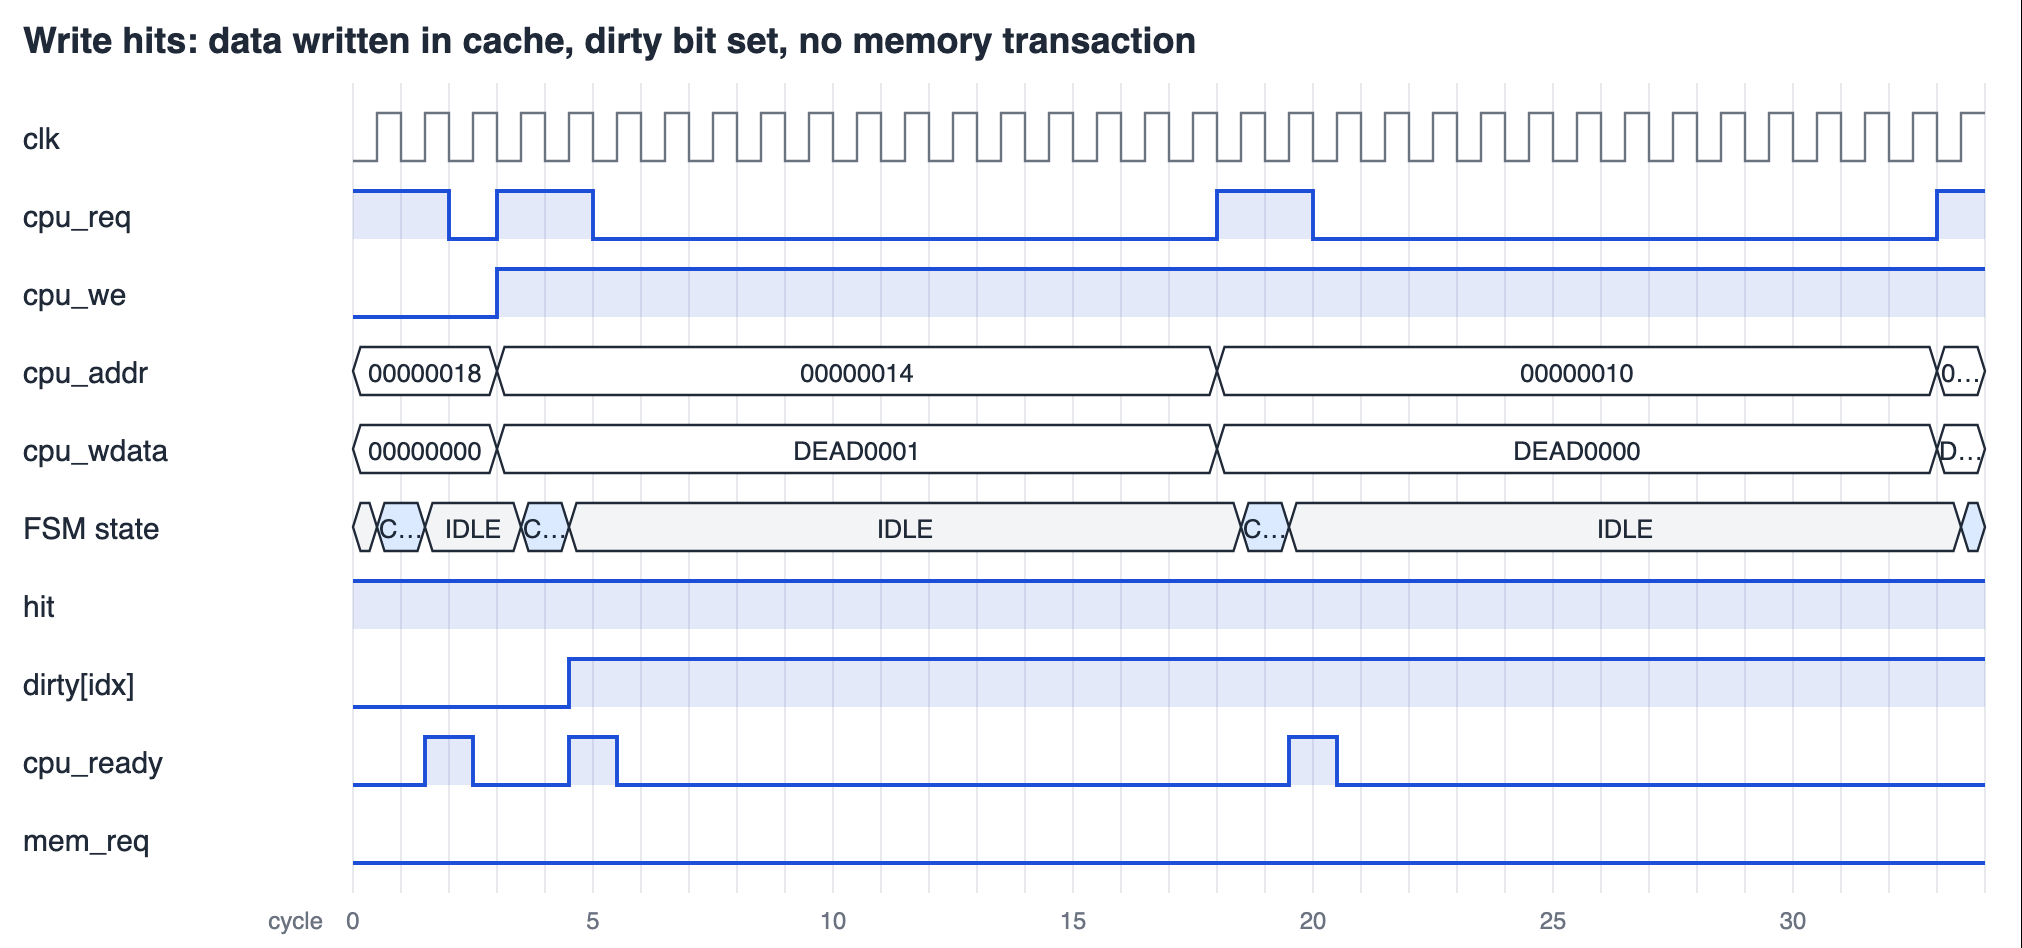
\includegraphics[width=0.49\textwidth]{fig_wave_writehit.png}\hfill
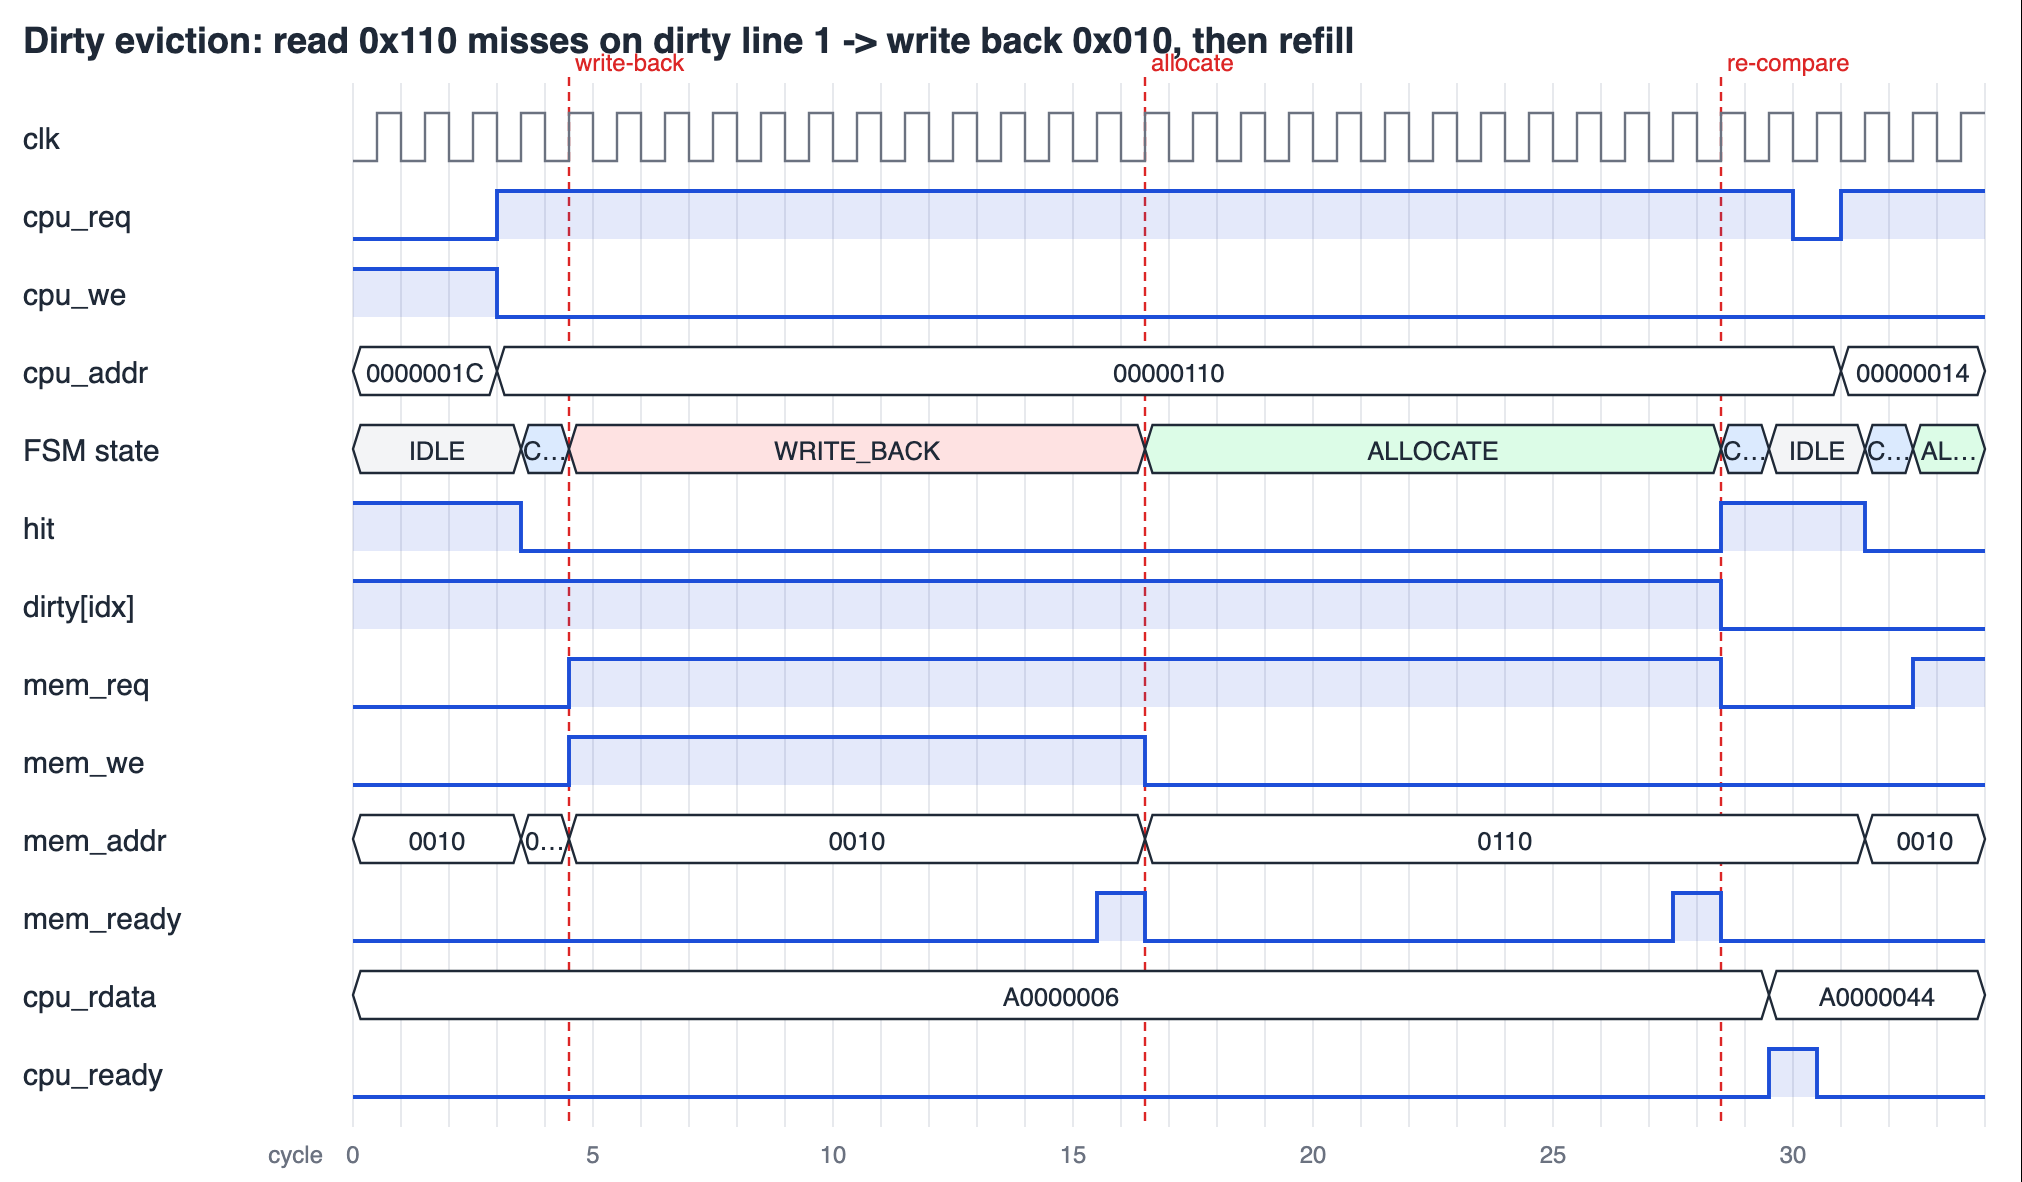
\includegraphics[width=0.49\textwidth]{fig_wave_evict.png}
\caption{Simulation waveforms. Left: write hits complete in two cycles, set
\texttt{dirty[idx]} and issue no memory request. Right: a read miss on dirty
line~1 writes victim block \texttt{0x010} back (\texttt{mem\_we}=1) \emph{before}
refilling block \texttt{0x110}. Dirty is cleared on refill, and the re-compare
hits and returns the correct word.}
\label{fig:wave}
\end{figure*}

Fig.~\ref{fig:wave} shows waveforms extracted from the VCD. A hit takes 2 cycles,
a clean miss 15 cycles, and a dirty miss 27 cycles (two 10-cycle memory
transactions plus handshakes).

\begin{table*}[t]
\caption{Preliminary Memory-Traffic Comparison (32-bit words moved; WB includes the final flush of lines still dirty)}
\label{tab:traffic}
\centering
\footnotesize
\begin{tabular}{@{}lrrrrrrr@{}}
\toprule
\textbf{Workload} & \textbf{Accesses} & \textbf{WB hit \%} & \textbf{WB write-backs}
 & \textbf{WB words} & \textbf{WT words} & \textbf{WB cycles} & \textbf{WT cycles} \\
\midrule
W1 Loop read-modify-write, 32 words $\times$8 & 512 & 98.4 & 0 & 64 & 288 & 1\,128 & 4\,200 \\
W2 Sequential read stream, 4\,KiB & 1\,024 & 75.0 & 0 & 1\,024 & 1\,024 & 5\,376 & 5\,376 \\
W3 Random 70\%R/30\%W, 2\,KiB & 1\,000 & 12.7 & 285 & 4\,648 & 2\,698 & 16\,769 & 13\,411 \\
W3b Random 70\%R/30\%W, 512\,B & 1\,000 & 48.6 & 221 & 2\,976 & 1\,683 & 11\,334 & 10\,051 \\
W4 Hot set 128\,B, 50\% writes & 1\,000 & 99.2 & 0 & 64 & 530 & 2\,104 & 8\,080 \\
W5 Sequential write stream, 4\,KiB & 1\,024 & 75.0 & 240 & 2\,048 & 1\,024 & 8\,256 & 14\,336 \\
W6 Conflict thrash (2 blocks, same index) & 256 & 0.0 & 255 & 2\,048 & 256 & 6\,900 & 3\,584 \\
\bottomrule
\end{tabular}
\end{table*}

\begin{figure}[t]
\centering
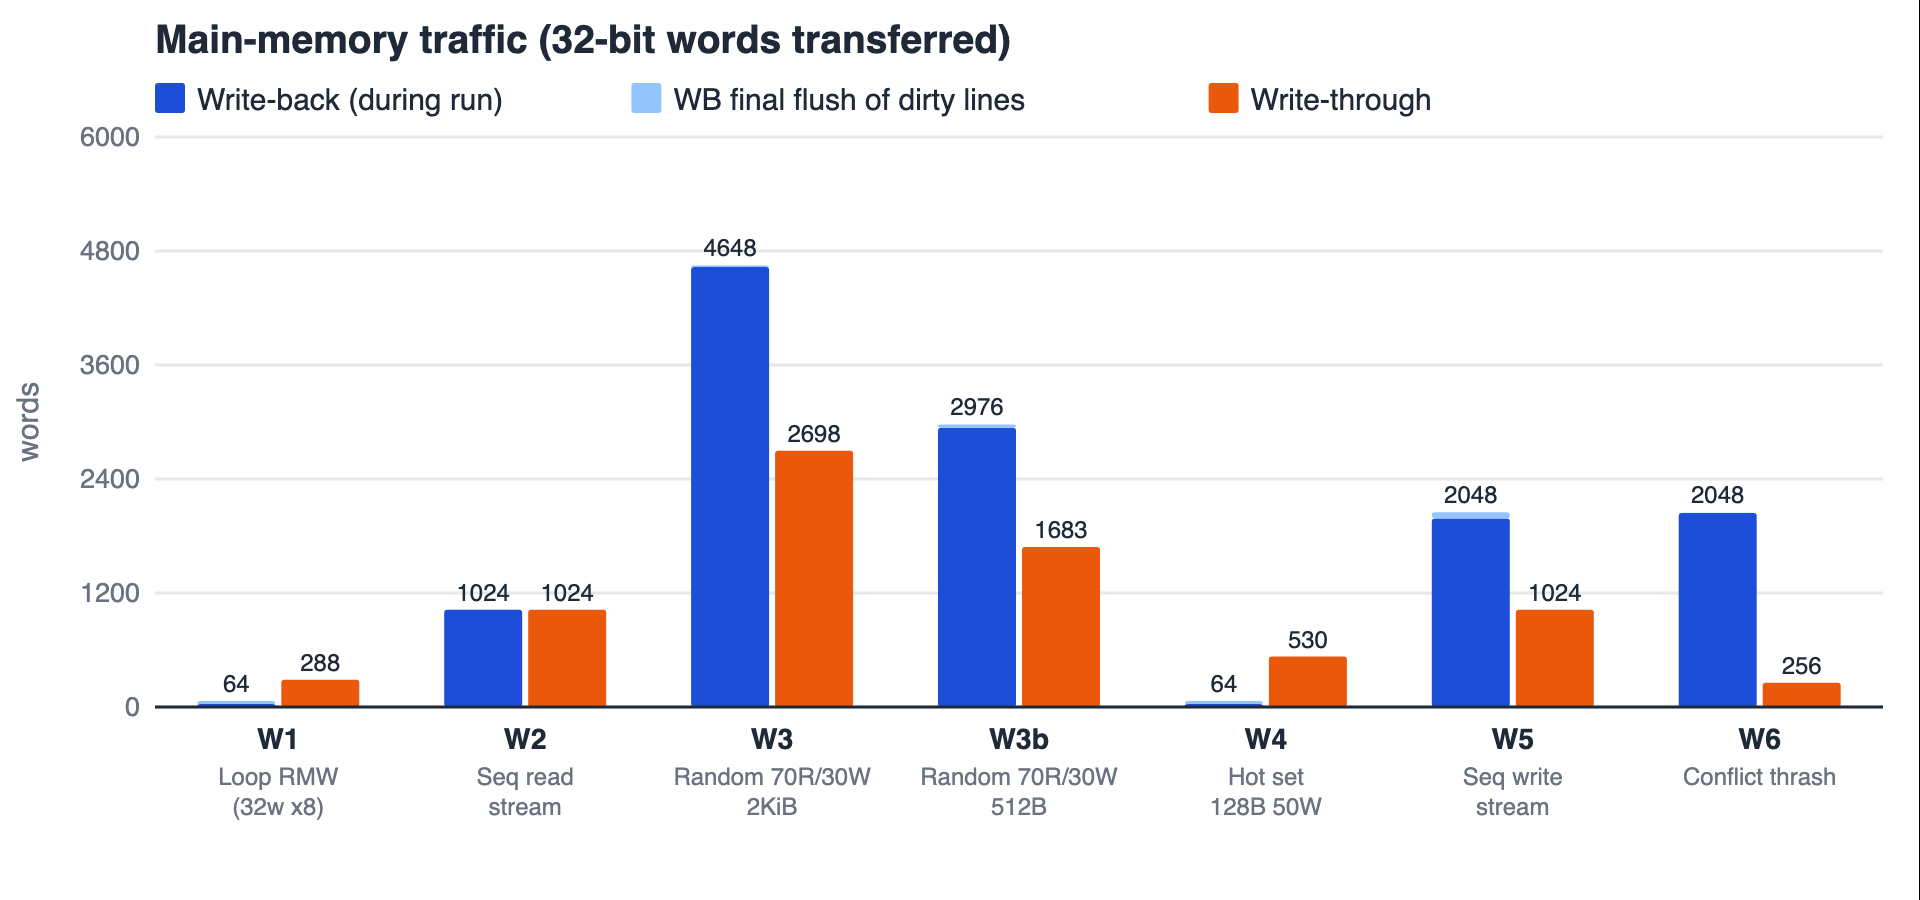
\includegraphics[width=\columnwidth]{fig_traffic.png}
\caption{Main-memory traffic per workload, write-back vs.\ write-through.}
\label{fig:traffic}
\end{figure}

Table~\ref{tab:traffic} and Fig.~\ref{fig:traffic} give a first traffic
comparison. With temporal write locality (W1, W4) the write-back cache cuts
traffic by 77.8\% and 87.9\% and runs 3.7--3.8$\times$ faster, because repeated
stores to a resident block cost nothing. Read-only streaming (W2) is identical
for both caches. Three cases favour write-through. In low-locality random
traffic (W3, W3b) most dirty blocks are evicted after few writes. In streaming
stores (W5) fetch-on-write reads every block before it is fully overwritten,
which Jouppi described~\cite{jouppi93}; WB still finishes 1.7$\times$ faster
because it stalls on block misses rather than on every store. In conflict
thrash (W6) every store evicts a dirty block (8 words vs.\ 1). These results
show that the controller behaves correctly and that write-back pays off only when
there is write locality.

\subsection{Plan for Phase II}
Phase II will (i)~add a no-fetch-on-write / write-validate option with
per-word dirty bits to remove the W5 penalty; (ii)~add a small write-back
buffer so that refill can start before the victim reaches memory; (iii)~evaluate
2-way set associativity with LRU against the W6 conflict case; and (iv)~report
synthesis area and timing.

% ----------------------------------------------------------------------------
\section{Individual Contributions}
\noindent\textit{(Each member's work is visible in the GitHub commit history.)}
\begin{itemize}
\item \textbf{Pankaj Upadhyay} -- Storage datapath: Cache Data RAM, Tag RAM,
Valid RAM, Dirty-Bit RAM, Tag Comparator; address mapping and
\texttt{cache\_params.vh}.
\item \textbf{Prakhar Rawat} -- Write-back controller FSM (\texttt{wb\_fsm.v}),
state diagram, and top-level integration (\texttt{wb\_cache\_top.v}).
\item \textbf{Harshit Kudhial} -- Memory interface, main-memory model with traffic
counters, and the write-through reference cache.
\item \textbf{Om Chimurkar} -- Self-checking testbench, golden model, directed
tests T0--T11, coherence checks, FSM coverage, waveform analysis.
\item \textbf{Vishuti Jamwal} -- Workload design, traffic and cycle analysis,
figure-generation scripts, literature review, IEEE report and demo video.
\end{itemize}

% ----------------------------------------------------------------------------
\begin{thebibliography}{10}

\bibitem{ph_cod}
D.~A. Patterson and J.~L. Hennessy, \emph{Computer Organization and Design:
The Hardware/Software Interface}, RISC-V ed., 2nd~ed.\hskip 1em plus 0.5em minus 0.4em
Cambridge, MA, USA: Morgan Kaufmann, 2020.

\bibitem{hp_quant}
J.~L. Hennessy and D.~A. Patterson, \emph{Computer Architecture: A Quantitative
Approach}, 6th~ed.\hskip 1em plus 0.5em minus 0.4em Cambridge, MA, USA: Morgan
Kaufmann, 2019.

\bibitem{smith82}
A.~J. Smith, ``Cache memories,'' \emph{ACM Comput. Surv.}, vol.~14, no.~3,
pp. 473--530, Sep. 1982.

\bibitem{goodman83}
J.~R. Goodman, ``Using cache memory to reduce processor-memory traffic,'' in
\emph{Proc. 10th Annu. Int. Symp. Comput. Archit. (ISCA)}, 1983, pp. 124--131.

\bibitem{jouppi93}
N.~P. Jouppi, ``Cache write policies and performance,'' in \emph{Proc. 20th
Annu. Int. Symp. Comput. Archit. (ISCA)}, 1993, pp. 191--201.

\bibitem{hill88}
M.~D. Hill, ``A case for direct-mapped caches,'' \emph{Computer}, vol.~21,
no.~12, pp. 25--40, Dec. 1988.

\bibitem{jouppi90}
N.~P. Jouppi, ``Improving direct-mapped cache performance by the addition of a
small fully-associative cache and prefetch buffers,'' in \emph{Proc. 17th Annu.
Int. Symp. Comput. Archit. (ISCA)}, 1990, pp. 364--373.

\bibitem{lee00}
H.-H.~S. Lee, G.~S. Tyson, and M.~K. Farrens, ``Eager writeback---A technique
for improving bandwidth utilization,'' in \emph{Proc. 33rd Annu. IEEE/ACM Int.
Symp. Microarchitecture (MICRO)}, 2000, pp. 11--21.

\bibitem{stuecheli10}
J.~Stuecheli, D.~Kaseridis, D.~Daly, H.~C. Hunter, and L.~K. John, ``The
virtual write queue: Coordinating DRAM and last-level cache policies,'' in
\emph{Proc. 37th Annu. Int. Symp. Comput. Archit. (ISCA)}, 2010, pp. 72--82.

\bibitem{jacob}
B.~Jacob, S.~W. Ng, and D.~T. Wang, \emph{Memory Systems: Cache, DRAM,
Disk}.\hskip 1em plus 0.5em minus 0.4em Burlington, MA, USA: Morgan Kaufmann,
2008.

\bibitem{ieee1364}
\emph{IEEE Standard for Verilog Hardware Description Language}, IEEE Std
1364-2005, 2006.

\bibitem{icarus}
S.~Williams, ``Icarus Verilog,'' 2024. [Online]. Available:
\url{https://steveicarus.github.io/iverilog/}

\end{thebibliography}

\end{document}
